\documentclass[conference]{IEEEtran}
\IEEEoverridecommandlockouts
\usepackage{cite}
\usepackage{amsmath,amssymb,amsfonts}
\usepackage{algorithmic}
\usepackage{graphicx}
\graphicspath{{../}}
\usepackage{textcomp}
\usepackage{xcolor}
\usepackage{booktabs}
\usepackage{multirow}
\usepackage{url}

% ---------------------------------------------------------------------------
% Drafting helpers. Remove \todo uses before submission; set \showtodosfalse
% to hide them in a review build.
% ---------------------------------------------------------------------------
\newif\ifshowtodos
\showtodostrue
\newcommand{\todo}[1]{\ifshowtodos\textcolor{red}{[TODO: #1]}\fi}
\newcommand{\verified}[1]{#1}  % wraps numbers already re-run and checked

\def\BibTeX{{\rm B\kern-.05em{\sc i\kern-.025em b}\kern-.08em
    T\kern-.1667em\lower.7ex\hbox{E}\kern-.125emX}}

\begin{document}

\title{Validated, yet Wrong: Four Ways Small-$n$ Metabolomics Machine Learning Passes Standard Checks\\
\thanks{Code, fixed partitions, and verification scripts: \todo{make repository public; github.com/Calvinkub/validated-yet-wrong, commit hash}.}}

\author{
\IEEEauthorblockN{Chaiyaporn Orrudee}
\IEEEauthorblockA{\textit{Artificial Intelligence Technology, School of Information Technology} \\
\textit{King Mongkut's Institute of Technology Ladkrabang}\\
Bangkok, Thailand \\
67070217@kmitl.ac.th}
\and
\IEEEauthorblockN{Kanin Calvin Shomwiwat}
\IEEEauthorblockA{\textit{Artificial Intelligence Technology, School of Information Technology} \\
\textit{King Mongkut's Institute of Technology Ladkrabang}\\
Bangkok, Thailand \\
67070015@kmitl.ac.th}
}

\maketitle

% ===========================================================================
\begin{abstract}
Small-cohort metabolomics studies routinely report near-perfect discrimination
after cross-validation, permutation testing, and feature-attribution checks.
We show, on public NMR data, four failure modes in which every one of these
standard checks passes while the reported result is wrong or uninterpretable:
(i) an outcome manufactured from the features through change scores,
(ii) exogenous contaminants that feature-removal faithfulness tests rank as
highly as genuine biology, (iii) a perfect acquisition-batch/label confound,
and (iv) a label whose name does not match what it encodes. For each, we give
the standard check it passes and the targeted control that exposes it. In a
bariatric-surgery responder forecast, a label-permutation test gave
$p=\verified{0.002}$, yet a pairing-destroyed null scored \emph{higher} than
the observed model, and after correcting the outcome the trained model
(PR-AUC \verified{0.483}) did no better than a learn-nothing baseline
(\verified{0.522}).
In simulation with no forecastable individual response, label permutation
rejected in 11--100\% of datasets at $\alpha=0.05$, rising with sample size;
residualising change on each marker's own baseline still rejected in
8--29\%, whereas residualising on all baselines jointly held the rate at
5--8\%. We release the controls as a
reusable checklist with reference code.
\end{abstract}

\begin{IEEEkeywords}
metabolomics, NMR, validation, data leakage, regression to the mean,
permutation test, feature attribution, batch effects, reproducibility
\end{IEEEkeywords}

% ===========================================================================
\section{Introduction}
\label{sec:intro}

% Para 1: the problem.
Machine-learning studies on small metabolomics cohorts ($n<200$) frequently
report AUC above 0.95. Readers are asked to trust these numbers because the
authors used cross-validation, a permutation test, and an explanation method
such as SHAP \cite{lundberg2017}. Yet leakage and related evaluation errors
have been documented across hundreds of ML-based studies in many fields
\cite{kapoor2023}, and omics data add hazards of their own: acquisition batch,
sample handling, and repeated measurements of the same person
\cite{leek2010}. With a few dozen subjects, any of these can produce a
near-perfect score.

% Para 2: the gap.
Each of these checks answers a narrow question. Cross-validation asks whether
the model generalises to new samples \emph{drawn the same way}; a label
permutation asks whether the features carry \emph{any} association with the
label; a faithfulness test asks whether the model \emph{relies} on a feature.
None asks whether the label measures what it claims to, or whether the
association is biological. A study can therefore pass all three checks and
still be wrong.

% Para 3: contributions.
This paper makes four contributions:
\begin{enumerate}
  \item A taxonomy of four failure modes, each paired with the standard check
        it passes and a targeted control that catches it
        (Table~\ref{tab:taxonomy}).
  \item A \emph{pairing-destroyed null} for change-score outcomes, shown to
        detect a manufactured outcome that label permutation accepts.
  \item A simulation study (36{,}000 datasets) showing that label permutation
        becomes \emph{more} wrong as $n$ grows, that the common per-marker
        regression-to-the-mean correction is itself liberal for correlated
        markers, and that joint residualisation restores near-nominal error.
  \item An open checklist and reference implementations of the controls for
        metabolomics ML studies.
\end{enumerate}

% ===========================================================================
\section{Related Work}
\label{sec:related}

\subsection{Regression to the mean and mathematical coupling}
Correlating change with initial value is a known statistical artefact
\cite{oldham1962, tu2007, barnett2005}, and a change score that shares terms
with the baseline is mathematically coupled to it \cite{archie1981}: measurement error and within-person
variation make extreme baselines move back toward the mean, so baseline
``predicts'' change even when nothing happens. The epidemiological remedies
(analysis of covariance, Oldham's method) are well known
\cite{vickers2001, glymour2005}. Our contribution is
not the artefact but its interaction with ML practice: an outcome
\emph{defined} from change scores, a flexible model given the baselines as
features, and a label permutation as the significance test. We show that this
combination certifies the artefact, and that the per-marker correction a
careful analyst might add is not sufficient.

\subsection{Leakage and confounding in ML-based science}
Kapoor and Narayanan \cite{kapoor2023} catalogue leakage types, including
features that act as proxies for the outcome and non-independence between
training and test data. Batch effects can be perfectly confounded with the
biological variable of interest, in which case no analysis can separate them
\cite{leek2010}; analytical bias in serum metabolomics is well documented
\cite{teahan2006, han2022}. Reporting guidelines such as TRIPOD+AI \cite{collins2024}
require that the outcome definition and its relation to the predictors be
stated. Our cases are concrete metabolomics instances of these categories,
each paired with a test that detects it.

\subsection{Feature-attribution faithfulness}
SHAP \cite{lundberg2017} attributes a prediction to features; ROAR
\cite{hooker2019} tests whether the attributed features matter by removing
them and retraining. Both answer a question about the \emph{model}. Attribution methods can mislead even about model behaviour
\cite{adebayo2018, kumar2020}. A feature
can be faithfully important to a model and still be an artefact of how the
samples were collected. We use a known exogenous contaminant as a positive
control to show that ROAR cannot tell the two apart.

\subsection{Permutation tests for classifiers}
A label permutation tests the null hypothesis that features and labels are
independent \cite{ojala2010}. Rejecting it shows only that \emph{some}
association exists. If the label is computed from the features, that
association is guaranteed, and the test answers a question nobody asked.
The permutation must also refit the model on every permuted label vector:
permuting labels against fixed out-of-fold scores is not a valid test
(Section~\ref{sec:sim}); the broader fragility of resampling-based
validation on small cohorts is well established
\cite{westerhuis2008, broadhurst2006, varma2006, varoquaux2018}.

% ===========================================================================
\section{Data and Common Setup}
\label{sec:data}

\subsection{Datasets}
\textbf{MTBLS242} \cite{mtbls242, gralka2015}: serum $^1$H-NMR from a
bariatric surgery cohort, released 10 Feb.\ 2017. The sample sheet lists 465
samples at five visits, labelled in its time-point factor as preoperative
(106), and 3, 6, 9 and 12 months after surgery (98, 98, 92 and 71);
21 metabolites are quantified. We re-downloaded the sheet from MetaboLights
on 15 Oct.\ 2026 and it is byte-identical to the copy used in all
experiments. Patient identifiers are not a column; they are recoverable from
sample names with the pattern \verb|^(\d+)[-_](\d+)[-_]S$| (one 6-month
sample, \verb|2_0242_2|, does not match and does not affect any analysis
here, which uses only the preoperative and 12-month visits). All 71
twelve-month patients also have a preoperative sample. The sheet records
neither the surgical procedure per sample nor any clinical covariate, although
the study design lists both gastric bypass and sleeve gastrectomy.

\textbf{MTBLS1} \cite{salek2007}: urine $^1$H-NMR, type 2 diabetes vs.\
control; 132 samples from 40--42 subjects (12 volunteers sampled at seven
time points; 28--30 patients whose sample-to-patient membership is not
deposited; see Section~\ref{sec:case3}).

\textbf{MTBLS881} \cite{maltesen2020}: serum $^1$H-NMR from 50 adults
undergoing cardiac surgery with cardiopulmonary bypass, sampled at six times
(from $-1$ to 20\,h) from two sites (left atrium, LA; pulmonary artery, PA).
We use it only to replicate Case~1 on a second cohort: 47 patients have both
the $-1$\,h and 20\,h samples at each site.

\subsection{Models and evaluation}
We deliberately reuse the models from the original analyses rather than
tuning new ones, since the point is to evaluate the checks, not the models.
Classifiers are XGBoost \cite{chen2016} with monotonic constraints whose
directions were assigned from the metabolomics literature (Cases 2--4) and
L2-penalised logistic regression (Case 1). The headline metric is PR-AUC
(average precision), reported next to the prevalence it must beat.
Cross-validation is repeated and grouped by subject wherever subjects can be
identified, and intervals come from bootstrap resampling of subjects. Every
analysis includes a learn-nothing baseline: a fixed, unfitted score that any
trained model must beat.

\begin{table*}[t]
\centering
\caption{Four failure modes: the standard check each passes and the control
that exposes it.}
\label{tab:taxonomy}
\footnotesize
\begin{tabular}{@{}c p{3.4cm} l l p{3.2cm} p{3.2cm}@{}}
\toprule
Case & Failure mode & Data & Reported result & Standard check passed & Exposing control \\
\midrule
1 & Outcome manufactured from features & MTBLS242 & PR-AUC 0.683 & Label permutation, $p=0.002$ & Pairing-destroyed null \\
2 & Contaminant ranked as biology & MTBLS242 & PR-AUC 0.972 & ROAR faithfulness & Known-artefact positive control \\
3 & Batch equals label & MTBLS1 & PR-AUC 0.976 & Subject-grouped CV & Metadata/batch audit \\
4 & Label name $\neq$ label meaning & MTBLS242 & ROC-AUC 0.973 & Subject-grouped CV & Label-provenance audit \\
\bottomrule
\end{tabular}
\end{table*}

% ===========================================================================
\section{Case 1: An Outcome Manufactured from the Features}
\label{sec:case1}

\subsection{Setup}
Task: predict from the preoperative profile whether a patient is a
twelve-month ``strong responder,'' defined as $\geq$9 of 11 markers changing
in the expected direction. 71 paired patients, 31 responders.

\subsection{Why the standard check passes}
Baseline $x_0$ is both the predictor and a term in the outcome
$\Delta = x_{12} - x_0$. Under pure noise, $\operatorname{corr}(x_0, \Delta)<0$
by construction; the observed median was \verified{$-0.62$}. A label
permutation breaks the label--feature link entirely, so it tests against a
null that the coupled outcome trivially beats: $p=\verified{0.002}$.

\subsection{Exposing control: pairing-destroyed null}
Shuffle which twelve-month sample belongs to which subject, recompute the
outcome from scratch, and refit. This keeps the arithmetic coupling and
removes any real individual-level signal. Because shuffling breaks the
positive correlation between visits, the null has \emph{stronger} coupling
than the observed data; the test is therefore conservative
(Section~\ref{sec:sim}) and is best read as a diagnostic: a model that does
not beat it has shown nothing beyond regression to the mean.

\subsection{Result}
\textbf{Original design} (raw change, $\geq$9 of 11 markers, contaminants
included). The trained model reaches PR-AUC \verified{0.683} against a
prevalence of \verified{0.437} (the originally reported \verified{0.671} does
not reproduce exactly on re-run, as the repository's own correction notes). A label
permutation with the model refitted on every permutation gives
$p=\verified{0.001}$ (\verified{0.002} with the original fixed-score
procedure). The pairing-destroyed null has median lift \verified{2.04$\times$}
and the observed lift is \verified{1.57$\times$}, below
\verified{499 of 500} null replicates (Fig.~\ref{fig:case1}). The model
cannot be distinguished from regression to the mean. In the original
solver the largest coefficient was \verified{0.018}, and an unfitted scorer
matched its PR-AUC to three decimals (\verified{0.653}).

\textbf{Corrected design} (change residualised on baseline inside each
training fold, contaminants removed). Two variants are shown in
Table~\ref{tab:case1}. In both, the trained model does not beat the
learn-nothing scorer, and refitted permutation tests give no evidence of
signal ($p=\verified{1.0}$). The repeat-level bootstrap interval for the gap
excludes zero on the wrong side, but it understates uncertainty by treating
repeats as independent; resampling the 71 subjects gives an interval that
spans zero. The defensible statement is that the model is \emph{no better
than} the scorer, not that it is worse.

\begin{table}[t]
\centering
\caption{Case 1, corrected designs. Gap = model $-$ learn-nothing scorer
PR-AUC; interval from a bootstrap over the 71 subjects. Prevalence differs
because the joint design yields a different responder count, so compare lifts
and gaps, not PR-AUC levels.}
\label{tab:case1}
\footnotesize
\begin{tabular}{@{}lrr@{}}
\toprule
 & Per-marker resid. & Joint resid. \\
\midrule
Responders / 71          & 31 & 37 \\
Prevalence               & 0.437 & 0.521 \\
Model PR-AUC             & 0.483 & 0.554 \\
Learn-nothing PR-AUC     & 0.522 & 0.589 \\
Gap                      & $-0.042$ & $-0.037$ \\
95\% interval            & [$-0.149$, $+0.052$] & [$-0.111$, $+0.037$] \\
Refit permutation $p$    & 1.000 & 1.000 \\
Pairing-null lift, median & 1.04 & 1.05 \\
\bottomrule
\end{tabular}
\end{table}

\begin{figure}[t]
\centering
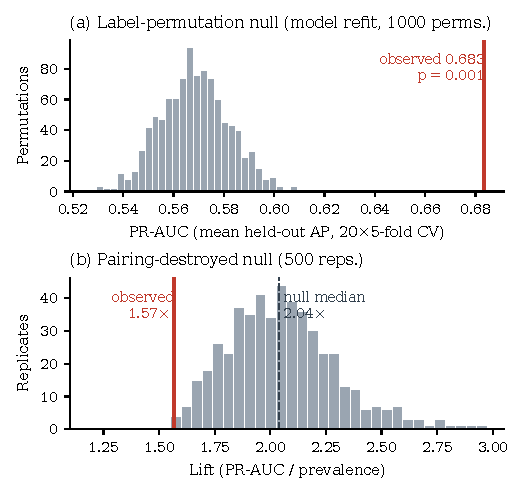
\includegraphics[width=\columnwidth]{figures/case1_nulls.pdf}
\caption{Original (withdrawn) design. (a) Label-permutation null of
average precision, model refitted per permutation. (b) Pairing-destroyed null
of lift. The label permutation rejects; the pairing-destroyed null sits above
the observed model.}
\label{fig:case1}
\end{figure}

\subsection{Replication on a second cohort}
We repeated the four tests on MTBLS881 with the design fixed in a
pre-registration file before any model was fitted: baseline $-1$\,h versus
20\,h; both sites analysed separately (LA declared primary); 11 marker
metabolites chosen in advance; improvement direction taken from training-fold
mean change only; $K$ chosen so prevalence is near 0.5; exogenous drugs
(propofol, heparin, ethanol) excluded. The model is unconstrained ridge
logistic regression with the same repeated CV as Case~1. This is a
different, acute setting (hours after surgery, not a year), so it tests the
statistical artefact, not the surgical biology. With 47 patients every
interval is wide (Table~\ref{tab:case1b}).

\textbf{Raw change replicates.} At both sites a label permutation rejects
($p=\verified{0.007}$), yet the pairing-destroyed null reaches equal or higher
lift (median \verified{1.49} and \verified{1.40} vs.\ observed
\verified{1.29} and \verified{1.19}), and the model does not beat the
learn-nothing scorer (gap \verified{$-0.037$} and \verified{$+0.013$}, both
intervals spanning zero). Refitting the full model on each shuffle puts the
observed lift inside the null ($p=\verified{0.86}$ at LA, \verified{0.91} at
PA; 150 replicates).

\textbf{Residualised outcomes replicate only partly.} At PA, joint
residualisation shows no signal ($p=\verified{0.977}$), matching MTBLS242. At
LA the per-marker outcome is permutation-significant ($p=\verified{0.003}$),
and for LA joint residualisation the permutation test is not significant
($p=\verified{0.103}$) while the model's lift (\verified{1.45}) exceeds the
scorer-based pairing-null 95th percentile (\verified{1.27}). The tests
disagree here, and 47 patients cannot resolve it. Every gap interval except
one (below) includes zero.

\textbf{Exogenous compounds create apparent signal.} Adding propofol, heparin
and ethanol to the features and markers made the joint-residualised outcome
permutation-significant at both sites ($p=\verified{0.005}$, the floor for
200 permutations), against $p=\verified{0.103}$ and \verified{0.977}
without them; at LA the gap became \verified{$+0.163$}
[\verified{$+0.069$}, \verified{$+0.252$}]. We did not test the mechanism,
but the pattern matches Case~2: drugs administered during surgery
distinguish samples because of handling, not metabolism.

\begin{table*}[t]
\centering
\caption{Case 1 replication on MTBLS881 ($n=47$ per site). Gap = model $-$
learn-nothing scorer PR-AUC, subject-bootstrap interval. $K$ = number of the
11 markers required to define a responder.}
\label{tab:case1b}
\footnotesize
\begin{tabular}{llrrrrrrr}
\toprule
Site & Outcome & Prev. & PR-AUC & Scorer & Gap [95\% CI] & $p_{\mathrm{perm}}$ & Lift & Pair-null lift \\
 & & & & PR-AUC & & (refit) & & med. (p95) \\
\midrule
LA & Raw change ($K{=}10$) & 0.49 & 0.632 & 0.695 & $-0.037$ [$-0.231$, $+0.118$] & 0.007 & 1.29 & 1.49 (2.09) \\
LA & Per-marker resid. ($K{=}6$) & 0.55 & 0.678 & 0.542 & $+0.164$ [$-0.004$, $+0.309$] & 0.003 & 1.23 & 1.05 (1.25) \\
LA & Joint resid. ($K{=}6$) & 0.43 & 0.619 & 0.545 & $+0.071$ [$-0.077$, $+0.190$] & 0.103 & 1.45 & 1.06 (1.27) \\
\midrule
PA & Raw change ($K{=}10$) & 0.64 & 0.757 & 0.723 & $+0.013$ [$-0.111$, $+0.154$] & 0.007 & 1.19 & 1.40 (1.89) \\
PA & Per-marker resid. ($K{=}6$) & 0.51 & 0.631 & 0.546 & $+0.078$ [$-0.086$, $+0.222$] & 0.096 & 1.24 & 1.05 (1.27) \\
PA & Joint resid. ($K{=}6$) & 0.53 & 0.598 & 0.629 & $-0.034$ [$-0.169$, $+0.092$] & 0.977 & 1.12 & 1.06 (1.23) \\
\bottomrule
\end{tabular}
\end{table*}

% ===========================================================================
\section{Case 2: Contaminants Ranked as Biology}
\label{sec:case2}

\subsection{Setup}
ROAR \cite{hooker2019} removes the top-$k$ attributed features, retrains, and
compares the score with removing $k$ random features. Here the attribution is
SHAP on the MTBLS242 pre- vs.\ 12-month task (177 samples, 21 metabolites).
We repeat the original analysis with three fixes: cross-validation is grouped
by patient (10 repeats of 5 folds), attribution is recomputed after every
retrain (recursive ROAR), and the random null uses 500 distinct draws per $k$
(exhaustive for $k\leq 2$) under the same folds as the informed runs.
Grouped baseline PR-AUC is \verified{0.973}; ungrouped CV gives
\verified{0.972}.

\subsection{Why the standard check passes}
Recursive ROAR removes, in order, dimethyl sulfone, isopropanol, L-valine,
glycine, methanol, and then further metabolites. From $k=3$ onward the
curve lies below almost the entire random band (null percentile
\verified{0.0--0.2}), so ROAR reports that the removed features genuinely
matter to the model. That is true. Dimethyl sulfone, isopropanol and methanol
are exogenous, and isopropanol is a skin-preparation agent used in surgery.
They distinguish pre- from post-operative samples because of how the samples
were handled, not because of metabolism.

\subsection{Exposing control: artefact vs.\ biology}
At $k=3$, removing the contaminant trio gives PR-AUC \verified{0.954}
(null percentile \verified{0.2}); removing three biological markers
(lipoproteins, L-valine, L-tyrosine) gives \verified{0.959} (percentile
\verified{1.2}). The \verified{0.006} gap is far smaller than the fold
standard deviation of about \verified{0.03}. ROAR cannot separate the two.

A spiked positive control makes the point without relying on this cohort.
We add a synthetic feature $d\,y + \mathcal{N}(0,1)$, which depends only on
the label and carries no biology, and run recursive ROAR (10 draws per $d$,
Table~\ref{tab:spike}). At $d=1.75$ the spike is ranked first by both SHAP
and ROAR, and removing it costs more than removing any real metabolite
(\verified{0.0127} vs.\ \verified{0.0073} for dimethyl sulfone). ROAR ranks a
feature by how much signal it carries, whatever its origin.

\begin{table}[t]
\centering
\caption{Spiked artefact: median rank among 22 features (1 = most
important).}
\label{tab:spike}
\footnotesize
\begin{tabular}{@{}rrr@{}}
\toprule
$d$ & SHAP rank & ROAR rank \\
\midrule
0.75 & 10 & 14.5 \\
1.25 & 3 & 3 \\
1.75 & 1 & 1 \\
\bottomrule
\end{tabular}
\end{table}

\begin{figure}[t]
\centering
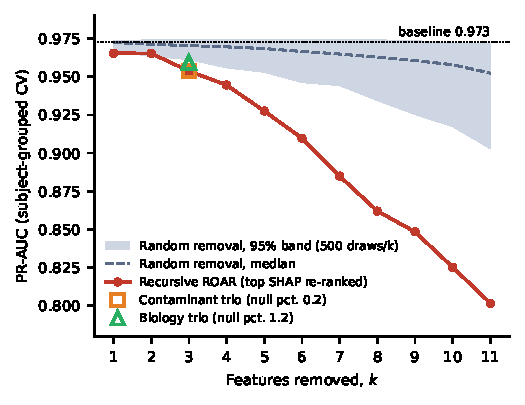
\includegraphics[width=\columnwidth]{figures/case2_roar.pdf}
\caption{Recursive ROAR on MTBLS242 against 500-draw random-removal bands.
The informed curve lies below the band from $k=3$ onward whether or not the
removed features are biological.}
\label{fig:case2}
\end{figure}

\subsection{Caveats}
This is one cohort, and its label is confounded with surgery (Case~4).
Random draws overlap and share folds, so percentiles below the band mean
``outside the random range,'' not calibrated $p$-values. Attribution used
all 177 samples, which makes informed removal slightly optimistic. The
multi-seed ranking places L-valine above lipoproteins, the reverse of the
original ranking; we kept the original biology trio for comparability.

% ===========================================================================
\section{Case 3: Batch Equals Label}
\label{sec:case3}
\subsection{Setup}
The Case~3 model is the original monotonic XGBoost on 132 urine spectra,
evaluated by CV grouped by subject. With seed 42 it reproduces the reported
PR-AUC of \verified{0.976}; over 20 CV seeds the mean is \verified{0.911}
(range \verified{0.845--0.975}), so the headline was a favourable split.

\subsection{Why the standard check passes}
Subject-grouped CV prevents the same person from appearing in training and
test folds. It cannot detect a confound shared by every member of a class.

\subsection{Exposing control: metadata audit}
We cross-tabulated the label against all 64 columns of the deposited sample
and assay sheets. Of these, 56 are constant (instrument, probe, pulse
sequence, temperature) and five are per-sample identifiers. Only sex varies
and is not an identifier. Every control sample name begins with
\verb|ADG19007u| and every diabetic sample name with \verb|ADG10003u|
(Table~\ref{tab:case3}). A logistic model given only this prefix, under the
same grouped CV, scores PR-AUC \verified{1.000} and ROC-AUC \verified{1.000}
against a prevalence of \verified{0.364}. No within-batch comparison is
possible because each batch contains one class. The deposited protocol also
gives the two groups different age and BMI criteria and different sampling
schedules (seven time points for volunteers vs.\ one to three for patients),
which are therefore aliased with the label as well.

Sex is imbalanced (controls \verified{66.7\%} male vs.\ cases
\verified{45.8\%}) but not confounded. Subject identity is not deposited: the
control numbering yields exactly 12 volunteers, matching the protocol, while
the 48 diabetic samples come from 28--30 patients whose sample-to-patient
membership cannot be recovered. A numbering heuristic used in our original
analysis merged at least three pairs of distinct patients. Merging errs
toward conservative CV, and ungrouped CV (\verified{0.969}) differs little,
so grouping does not drive the result; batch does, and it cannot be removed.

\begin{table}[t]
\centering
\caption{MTBLS1 samples by label, sample-name prefix and sex. The prefix
determines the label exactly; sex does not.}
\label{tab:case3}
\footnotesize
\begin{tabular}{@{}llrrrr@{}}
\toprule
Label & Prefix & F & M & Samples & Subjects \\
\midrule
Control & \texttt{ADG19007u} & 28 & 56 & 84 & 12 \\
T2DM    & \texttt{ADG10003u} & 26 & 22 & 48 & 28--30 \\
\midrule
Total   &                    & 54 & 78 & 132 & 40--42 \\
\bottomrule
\end{tabular}
\end{table}

% ===========================================================================
\section{Case 4: The Label Is Not What It Is Called}
\label{sec:case4}
The ``obese vs.\ non-obese'' task on MTBLS242 is in fact ``preoperative vs.\
twelve months after surgery'': \verified{71} of \verified{106} patients appear
in both classes. Subject-grouped CV (\verified{0.969}) and naive CV
(\verified{0.970}) agree, so the issue is not leakage but label meaning.
A classifier trained on this label learns everything that differs between a
patient before surgery and the same patient a year later: weight loss, but
also post-surgical diet, supplements and medication, fasting state, and the
year-long gap in sample storage. Its score is not evidence that the serum
profile identifies obesity in a general population, where lean and obese
people differ in age, sex and lifestyle rather than in surgical history. The
correct description is ``pre- vs.\ post-bariatric-surgery classification,''
and the check that exposes the mismatch is not statistical: write down, in one
sentence, what physically distinguishes the two classes.

% ===========================================================================
\section{Simulation Study}
\label{sec:sim}

\subsection{Design}
Each subject $i$ has a persistent level $\mu_{ij}$ for $p=11$ outcome markers,
with a shared factor (inter-marker correlation $\rho=0.3$), and ten auxiliary
features $z_i\sim\mathcal{N}(0,I)$. Observed visits are
\begin{align}
x^{(0)}_{ij} &= \sqrt{r}\,\mu_{ij} + \sqrt{1-r}\,\varepsilon^{(0)}_{ij},\\
x^{(12)}_{ij} &= \sqrt{r}\,(\mu_{ij} + \gamma\, g_i\, s_j) + \sqrt{1-r}\,\varepsilon^{(12)}_{ij},
\end{align}
where $r$ is the reliability (share of variance that persists between
visits), $s_j\in\{\pm1\}$ the expected direction of marker $j$, and
$g_i = w^\top z_i/\lVert w\rVert$ a forecastable response propensity. With
$\gamma=0$ no individual response exists, so any association between baseline
and outcome is regression to the mean. The outcome is the MTBLS242-style rule
``$\geq$6 of 11 markers change in the expected direction.'' The model is
ridge regression ($\lambda=10$) on the 21 standardised baseline features,
scored out-of-fold in 5-fold CV by average precision.

We vary $n\in\{50,100,200,500\}$, $r\in\{0.25,0.5,0.75\}$ and
$\gamma\in\{0,0.25,0.5\}$, with 1{,}000 datasets per cell. Setting $r=0.25$
reproduces the median baseline--change correlation of $-0.62$ observed in
MTBLS242. Each dataset is tested four ways at $\alpha=0.05$, each with 200
null replicates and the model refitted on every replicate:
\begin{enumerate}
  \item \textbf{Label permutation} on the raw-change outcome.
  \item \textbf{Pairing-destroyed null} on lift (AP over prevalence).
  \item \textbf{Per-marker residualisation}: within each training fold,
        regress change$_j$ on baseline$_j$; label from residuals; permute.
  \item \textbf{Joint residualisation}: as (3), but regress change$_j$ on all
        11 baselines.
\end{enumerate}
A permutation test that holds out-of-fold scores fixed and permutes only the
labels rejected 9.7\% of pure-noise datasets in our sanity check; refitting
on each permutation \cite{ojala2010} gave 5.3\%, so all tests refit.

\subsection{Results}
Table~\ref{tab:sim} and Fig.~\ref{fig:sim} give the rejection rates.

\textbf{Label permutation is wrong, and more so with more data.} With no
individual response, it rejected in 26\% of datasets at $n=50$ and 100\% at
$n=500$ when $r=0.25$; even at $r=0.75$ it reached 90\% at $n=500$.
More subjects estimate the regression-to-the-mean artefact more precisely;
they do not remove it.

\textbf{Per-marker residualisation is not enough.} Residualising each
marker's change on its own baseline left false-positive rates of 8--29\%,
again rising with $n$. When markers are correlated, residual change in
marker $j$ remains correlated with the baselines of the other markers,
which the model also sees.

\textbf{Joint residualisation is near nominal.} Regressing each change on all
baselines kept the rate at 5.3--8.1\%, slightly liberal at $n=50$, while
retaining power similar to label permutation when a real response exists
(e.g.\ 97.5\% vs.\ 100\% at $\gamma=0.25$, $r=0.25$, $n=500$).

\textbf{The pairing-destroyed null is valid but conservative.} Its
false-positive rate never exceeded 4.3\%, but at the MTBLS242-like reliability
$r=0.25$ and $\gamma=0.25$ it had no power at any $n$ (4--5\%). It detects
manufactured outcomes; it should not be the only test of a real one.

\begin{table}[t]
\centering
\caption{False-positive rate (\%) with no individual response ($\gamma=0$),
$\alpha=0.05$, 1{,}000 datasets per row. Wilson 95\% half-width $\leq$3.1
points.}
\label{tab:sim}
\footnotesize
\begin{tabular}{@{}rr rrrr@{}}
\toprule
$r$ & $n$ & Label perm. & Pair-null & Per-marker & Joint \\
\midrule
0.25 & 50  & 26.1  & 4.3 & 8.0  & 7.4 \\
0.25 & 100 & 52.0  & 2.1 & 9.3  & 6.2 \\
0.25 & 200 & 92.6  & 0.7 & 12.0 & 5.9 \\
0.25 & 500 & 100.0 & 0.3 & 18.9 & 6.3 \\
0.50 & 50  & 16.3  & 2.2 & 10.9 & 8.1 \\
0.50 & 100 & 35.9  & 0.6 & 13.1 & 6.9 \\
0.50 & 200 & 74.4  & 0.2 & 16.3 & 6.8 \\
0.50 & 500 & 99.6  & 0.0 & 28.8 & 6.7 \\
0.75 & 50  & 10.6  & 0.9 & 9.6  & 6.4 \\
0.75 & 100 & 18.8  & 0.2 & 13.3 & 6.7 \\
0.75 & 200 & 40.4  & 0.0 & 16.2 & 6.5 \\
0.75 & 500 & 90.3  & 0.0 & 27.0 & 5.3 \\
\bottomrule
\end{tabular}
\end{table}

\begin{figure*}[t]
\centering
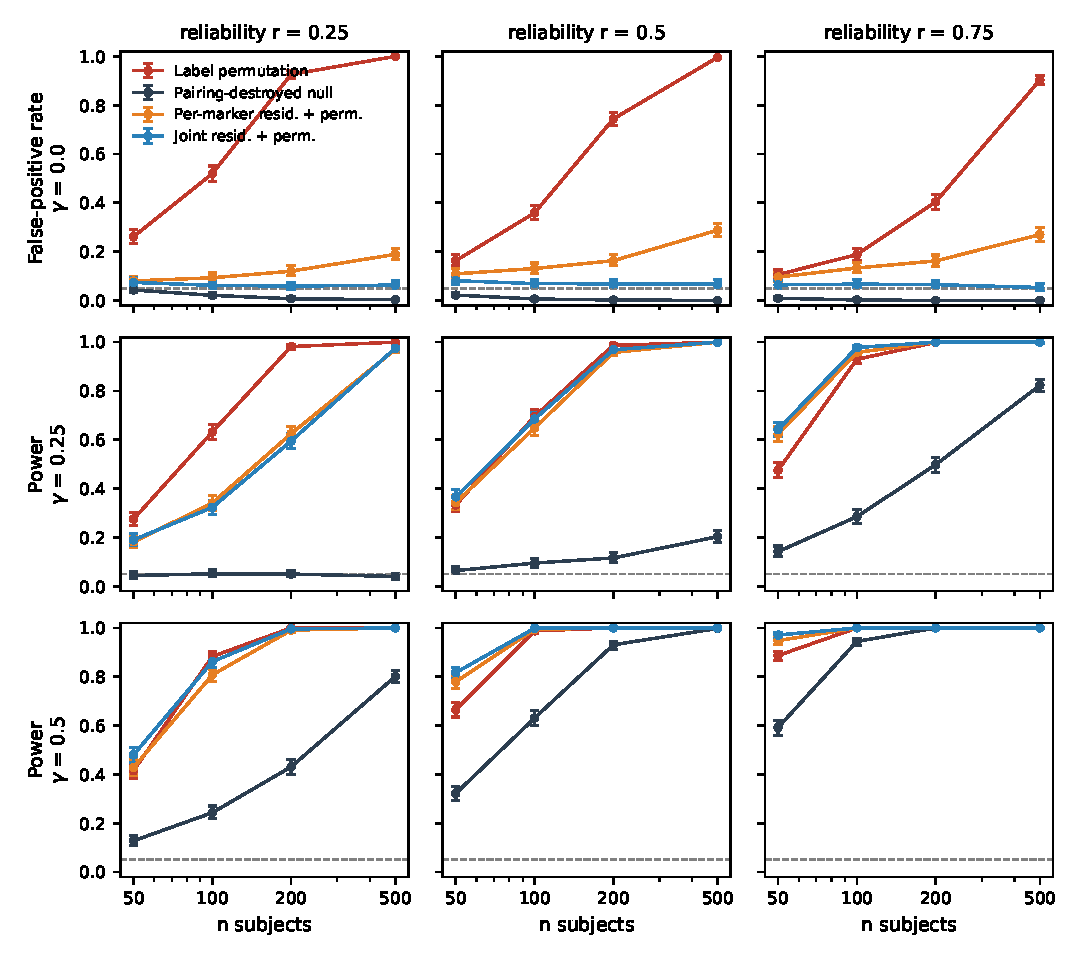
\includegraphics[width=0.82\textwidth]{figures/sim_rejection.pdf}
\caption{Rejection rate vs.\ number of subjects. Top row: false-positive rate
with no individual response ($\gamma=0$). Lower rows: power with a real,
forecastable response. Columns: reliability $r$. Dashed line: $\alpha=0.05$.
Error bars: Wilson 95\% intervals over 1{,}000 datasets.}
\label{fig:sim}
\end{figure*}

\subsection{Implication for Case 1}
The per-marker correction used in the original analysis is liberal, so
Section~\ref{sec:case1} repeats the corrected analysis with joint
residualisation. The conclusion is unchanged: the model does no better than
an unfitted scorer ($p=1.0$ with refitting). A liberal test that finds
nothing, followed by a better-calibrated test that also finds nothing, is
consistent evidence of absence at this sample size.

% ===========================================================================
\section{Discussion}
\label{sec:discussion}

\subsection{A checklist for small-$n$ metabolomics ML}
\begin{enumerate}
  \item If the outcome is computed from the features, do not rely on a
        label permutation. Residualise change on \emph{all} baselines inside
        each training fold, and report a pairing-destroyed null as a
        diagnostic.
  \item Refit the model inside every permutation replicate.
  \item Include a learn-nothing baseline and report the gap with an interval.
  \item Audit features for exogenous compounds; report results with and
        without them.
  \item Cross-tabulate the label against every metadata column (batch, run
        order, sample-name prefix, sex).
  \item State in one sentence what the label physically encodes.
\end{enumerate}

\subsection{Limitations}
The empirical cases use three small public datasets, chosen because their
problems are verifiable from the published files. The findings concern
validation practice; they say nothing for or against the biology of obesity
or diabetes. Regression to the mean is classical statistics, and our
contribution is limited to showing how ML practice fails to detect it. The
simulation uses Gaussian data, a linear ridge model and one outcome rule;
non-linear models and other rules may differ in degree. The pairing-destroyed
null is conservative and can miss real effects at low reliability, so it
should be a diagnostic, not the sole test. Finally, the joint residualisation
removes any \emph{true} biological dependence of change on baseline together
with the artefact; separating the two needs repeated baseline measurements.

% ===========================================================================
\section{Conclusion}
\label{sec:conclusion}
Cross-validation, permutation tests and attribution checks are necessary but
answer narrow questions. In four public-data cases, each passed while the
result was wrong: an outcome built from its own features, contaminants ranked
as biology, a batch equal to the label, and a label named for something it
did not measure. Each failure has a cheap, targeted control. We recommend
that small-$n$ metabolomics ML studies report these controls alongside their
headline score, and we release code that runs them.

% ===========================================================================
\section*{Data and Code Availability}
MTBLS242, MTBLS1 and MTBLS881 are public through MetaboLights \cite{haug2020}.
\todo{Repository URL, commit, test-suite instructions.}

\section*{Acknowledgment}
\todo{Funding, advisors.}

\section*{Use of Generative AI}
The authors used Claude (Anthropic) to assist with analysis code, the
simulation, and drafting text. The authors reviewed all code and text,
re-ran every reported analysis, and take full responsibility for the
content. \todo{Adjust wording to the target venue's policy.}

% ===========================================================================
\begin{thebibliography}{00}
\bibitem{mtbls242} EMBL-EBI, ``MetaboLights study MTBLS242: Metabolomic fingerprint of severe obesity is dynamically affected by bariatric surgery in a procedure-dependent manner,'' dataset. [Online]. Available: \url{https://www.ebi.ac.uk/metabolights/MTBLS242}
\bibitem{gralka2015} E. Gralka, C. Luchinat, L. Tenori, B. Ernst, M. Thurnheer, and B. Schultes, ``Metabolomic fingerprint of severe obesity is dynamically affected by bariatric surgery in a procedure-dependent manner,'' \textit{Am. J. Clin. Nutr.}, vol. 102, no. 6, pp. 1313--1322, Dec. 2015, doi: 10.3945/ajcn.115.110536.
\bibitem{salek2007} R. M. Salek \textit{et al.}, ``A metabolomic comparison of urinary changes in type 2 diabetes in mouse, rat, and human,'' \textit{Physiol. Genomics}, vol. 29, no. 2, pp. 99--108, Apr. 2007, doi: 10.1152/physiolgenomics.00194.2006.
\bibitem{haug2020} K. Haug \textit{et al.}, ``MetaboLights: a resource evolving in response to the needs of its scientific community,'' \textit{Nucleic Acids Res.}, vol. 48, no. D1, pp. D440--D444, Jan. 2020, doi: 10.1093/nar/gkz1019.
\bibitem{oldham1962} P. D. Oldham, ``A note on the analysis of repeated measurements of the same subjects,'' \textit{J. Chronic Dis.}, vol. 15, no. 10, pp. 969--977, 1962, doi: 10.1016/0021-9681(62)90116-9.
\bibitem{tu2007} Y.-K. Tu and M. S. Gilthorpe, ``Revisiting the relation between change and initial value: a review and evaluation,'' \textit{Stat. Med.}, vol. 26, no. 2, pp. 443--457, Jan. 2007, doi: 10.1002/sim.2538.
\bibitem{barnett2005} A. G. Barnett, J. C. van der Pols, and A. J. Dobson, ``Regression to the mean: what it is and how to deal with it,'' \textit{Int. J. Epidemiol.}, vol. 34, no. 1, pp. 215--220, Feb. 2005, doi: 10.1093/ije/dyh299.
\bibitem{kapoor2023} S. Kapoor and A. Narayanan, ``Leakage and the reproducibility crisis in machine-learning-based science,'' \textit{Patterns}, vol. 4, no. 9, Art. no. 100804, Sep. 2023, doi: 10.1016/j.patter.2023.100804.
\bibitem{leek2010} J. T. Leek \textit{et al.}, ``Tackling the widespread and critical impact of batch effects in high-throughput data,'' \textit{Nat. Rev. Genet.}, vol. 11, no. 10, pp. 733--739, Oct. 2010, doi: 10.1038/nrg2825.
\bibitem{collins2024} G. S. Collins \textit{et al.}, ``TRIPOD+AI statement: updated guidance for reporting clinical prediction models that use regression or machine learning methods,'' \textit{BMJ}, vol. 385, Art. no. e078378, 2024, doi: 10.1136/bmj-2023-078378.
\bibitem{hooker2019} S. Hooker, D. Erhan, P.-J. Kindermans, and B. Kim, ``A benchmark for interpretability methods in deep neural networks,'' in \textit{Proc. Adv. Neural Inf. Process. Syst. (NeurIPS)}, vol. 32, 2019.
\bibitem{lundberg2017} S. M. Lundberg and S.-I. Lee, ``A unified approach to interpreting model predictions,'' in \textit{Proc. Adv. Neural Inf. Process. Syst. (NeurIPS)}, vol. 30, 2017.
\bibitem{ojala2010} M. Ojala and G. C. Garriga, ``Permutation tests for studying classifier performance,'' \textit{J. Mach. Learn. Res.}, vol. 11, pp. 1833--1863, 2010.
\bibitem{chen2016} T. Chen and C. Guestrin, ``XGBoost: A scalable tree boosting system,'' in \textit{Proc. 22nd ACM SIGKDD Int. Conf. Knowl. Discov. Data Min.}, 2016, pp. 785--794, doi: 10.1145/2939672.2939785.
\bibitem{archie1981} J. P. Archie, ``Mathematic coupling of data: a common source of error,'' \textit{Ann. Surg.}, vol. 193, no. 3, pp. 296--303, Mar. 1981, doi: 10.1097/00000658-198103000-00008.
\bibitem{vickers2001} A. J. Vickers and D. G. Altman, ``Analysing controlled trials with baseline and follow up measurements,'' \textit{BMJ}, vol. 323, no. 7321, pp. 1123--1124, 2001, doi: 10.1136/bmj.323.7321.1123.
\bibitem{glymour2005} M. M. Glymour, J. Weuve, L. F. Berkman, I. Kawachi, and J. M. Robins, ``When is baseline adjustment useful in analyses of change? An example with education and cognitive change,'' \textit{Am. J. Epidemiol.}, vol. 162, no. 3, pp. 267--278, Aug. 2005, doi: 10.1093/aje/kwi187.
\bibitem{teahan2006} O. Teahan \textit{et al.}, ``Impact of analytical bias in metabonomic studies of human blood serum and plasma,'' \textit{Anal. Chem.}, vol. 78, no. 13, pp. 4307--4318, Jul. 2006, doi: 10.1021/ac051972y.
\bibitem{han2022} W. Han and L. Li, ``Evaluating and minimizing batch effects in metabolomics,'' \textit{Mass Spectrom. Rev.}, vol. 41, no. 3, pp. 421--442, 2022, doi: 10.1002/mas.21672.
\bibitem{adebayo2018} J. Adebayo, J. Gilmer, M. Muelly, I. Goodfellow, M. Hardt, and B. Kim, ``Sanity checks for saliency maps,'' in \textit{Proc. Adv. Neural Inf. Process. Syst. (NeurIPS)}, vol. 31, 2018.
\bibitem{kumar2020} I. E. Kumar, S. Venkatasubramanian, C. Scheidegger, and S. Friedler, ``Problems with Shapley-value-based explanations as feature importance measures,'' in \textit{Proc. 37th Int. Conf. Mach. Learn. (ICML)}, PMLR vol. 119, 2020, pp. 5491--5500.
\bibitem{vandersar2015} S. A. van der Sar \textit{et al.}, ``Ethanol contamination of cerebrospinal fluid during standardized sampling and its effect on $^1$H-NMR metabolomics,'' \textit{Anal. Bioanal. Chem.}, vol. 407, no. 16, pp. 4835--4839, Jun. 2015, doi: 10.1007/s00216-015-8663-9.
\bibitem{bernini2011} P. Bernini, I. Bertini, C. Luchinat, P. Nincheri, S. Staderini, and P. Turano, ``Standard operating procedures for pre-analytical handling of blood and urine for metabolomic studies and biobanks,'' \textit{J. Biomol. NMR}, vol. 49, no. 3--4, pp. 231--243, 2011, doi: 10.1007/s10858-011-9489-1.
\bibitem{westerhuis2008} J. A. Westerhuis \textit{et al.}, ``Assessment of PLSDA cross validation,'' \textit{Metabolomics}, vol. 4, no. 1, pp. 81--89, 2008, doi: 10.1007/s11306-007-0099-6.
\bibitem{varma2006} S. Varma and R. Simon, ``Bias in error estimation when using cross-validation for model selection,'' \textit{BMC Bioinformatics}, vol. 7, Art. no. 91, 2006, doi: 10.1186/1471-2105-7-91.
\bibitem{varoquaux2018} G. Varoquaux, ``Cross-validation failure: Small sample sizes lead to large error bars,'' \textit{NeuroImage}, vol. 180, pp. 68--77, 2018, doi: 10.1016/j.neuroimage.2017.06.061.
\bibitem{broadhurst2006} D. I. Broadhurst and D. B. Kell, ``Statistical strategies for avoiding false discoveries in metabolomics and related experiments,'' \textit{Metabolomics}, vol. 2, no. 4, pp. 171--196, 2006, doi: 10.1007/s11306-006-0037-z.
\bibitem{maltesen2020} R. G. Maltesen, R. Wimmer, and B. S. Rasmussen, ``A longitudinal serum NMR-based metabolomics dataset of ischemia-reperfusion injury in adult cardiac surgery,'' \textit{Sci. Data}, vol. 7, Art. no. 198, 2020, doi: 10.1038/s41597-020-0545-0.
\end{thebibliography}

\end{document}
